\documentclass[12pt,oneside,openany,a4paper]{book}

\usepackage{geometry}
\geometry{textheight=20.5cm,top=3cm,bottom=3cm,footskip=1.5cm,
marginparwidth=2.5cm,left=3cm,right=3cm}
\usepackage{fontspec}

% 設定中文和英文的字體
\setmainfont{Times New Roman} % 設定英文為 Times New Roman
\usepackage{xeCJK}
\setCJKmainfont{標楷體} % 設定中文為 標楷體
\XeTeXlinebreaklocale "zh"
\XeTeXlinebreakskip = 0pt plus 1pt

% 啟用自動換行和微調
\usepackage{microtype}

% 章、節、小節名稱設定
\usepackage[small,sf,center]{titlesec}
\titleformat{\chapter}[hang]{\centering\Large\rm}{}{0.2cm}{}
\titlespacing{\chapter}{0cm}{5mm}{5mm}
\titleformat{\section}[hang]{\large\rm}{}{0.2cm}{}
\titlespacing{\section}{0cm}{3mm}{5mm}
\titleformat{\subsection}[hang]{\normalsize\rm}{}{0.3cm}{}
\titlespacing{\subsection}{0.5cm}{0.2cm}{0.2cm}
\renewcommand{\chaptername}{}
\renewcommand{\thechapter}{}
\renewcommand{\thesection}{}
\renewcommand{\thesubsection}{}
% 設定各目次的標題
\usepackage{titletoc}
\renewcommand{\contentsname}{目錄}
\renewcommand{\listfigurename}{圖目次}
\renewcommand{\listtablename}{表目次}

% 設定圖表標題和排序方式
\usepackage{caption}
\renewcommand{\figurename}{圖}
\renewcommand{\tablename}{表}
\renewcommand{\thetable}{\arabic{chapter}.\arabic{table}}
\renewcommand{\thefigure}{\arabic{chapter}.\arabic{figure}}

% 附錄標題
\usepackage{appendix}
\renewcommand{\appendixpagename}{\Large 附錄}

\usepackage{url}
\def\UrlFont{\rm}
% PDF 超連結套件
\usepackage[colorlinks=true,urlcolor=blue,bookmarks=false]{hyperref}

% 插圖套件
\usepackage{graphicx}

% 特殊符號與數學套件
\usepackage{pifont}
\usepackage{amsthm}
\usepackage{amsmath,amssymb}

\begin{document}
% 內文基本設定
\pagestyle{plain}
\parindent=0.8cm

\pagenumbering{gobble}
% 封面
\newpage
\thispagestyle{empty}
\begin{titlepage}
    \begin{center}
        {\LARGE
            國立中興大學資訊工程學系\\
            碩士學位論文
        }
        \vspace{4.8cm}

        {\huge
            (中   文   論   文   題   目)
        }
        \vspace{2cm}

        {\LARGE
            (英   文   論   文   題   目)
        }
        \vspace{6.2cm}

        {\LARGE
            \begin{tabular}{lr}
                \makebox[4em][s]{指導教授}:\makebox[3em][s]{X\hspace{\fill}X\hspace{\fill}X}\\
                \makebox[4em][s]{研\hspace{\fill}究\hspace{\fill}生}:\makebox[3em][s]{X\hspace{\fill}X\hspace{\fill}X}
            \end{tabular}
        }
        \vspace{2.9cm}

        {\LARGE
            中華民國XX年XX月
        }
    \end{center}
\end{titlepage}


% 空白頁(題贈用)
\newpage
\thispagestyle{empty}
\begin{center}
\end{center}

% 書名頁(中文)
\newpage
\thispagestyle{empty}
\begin{titlepage}
    \begin{center}
        {\LARGE
            國立中興大學資訊工程學系\\
            碩士學位論文
        }
        \vspace{4.8cm}

        {\huge
            (中   文   論   文   題   目)
        }
        \vspace{2cm}

        {\LARGE
            (英   文   論   文   題   目)
        }
        \vspace{6.2cm}

        {\LARGE
            \begin{tabular}{lr}
                \makebox[4em][s]{指導教授}:\makebox[3em][s]{X\hspace{\fill}X\hspace{\fill}X}\\
                \makebox[4em][s]{研\hspace{\fill}究\hspace{\fill}生}:\makebox[3em][s]{X\hspace{\fill}X\hspace{\fill}X}
            \end{tabular}
        }
        \vspace{2.9cm}

        {\LARGE
            中華民國XX年XX月
        }
    \end{center}
\end{titlepage}


% 審核頁
\begin{center}
    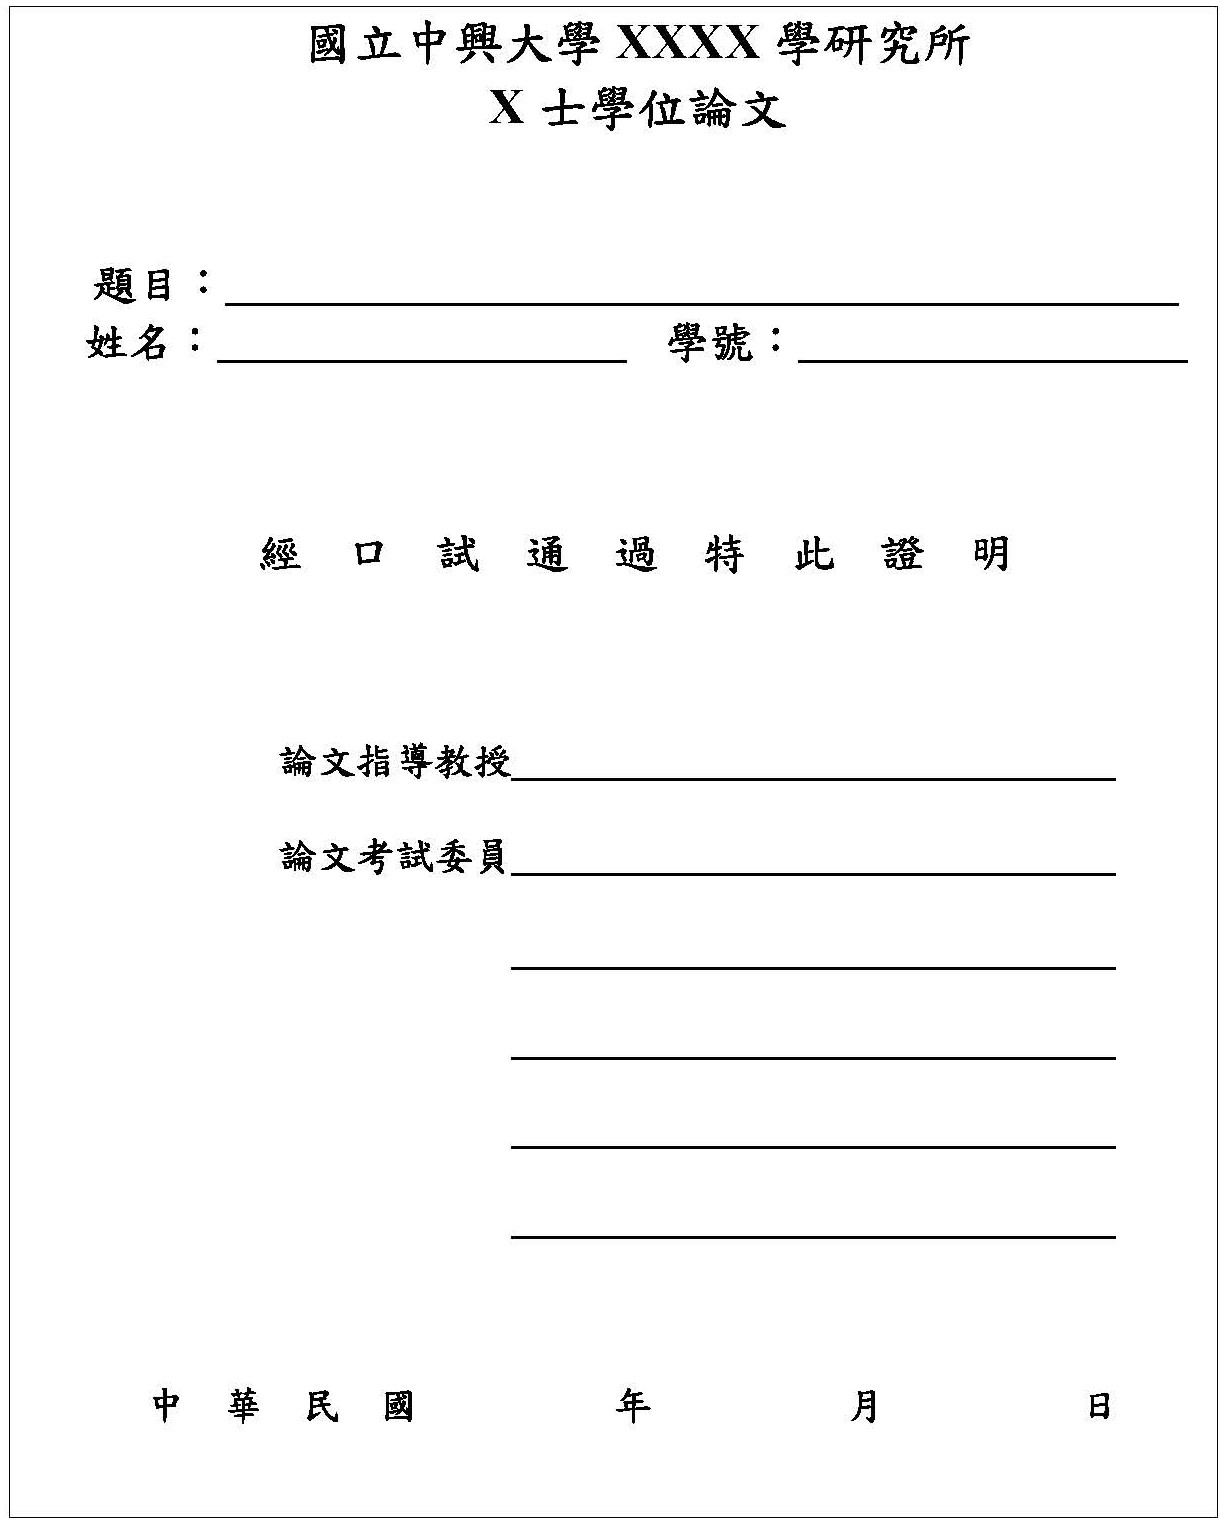
\includegraphics[bb=0 0 1224 1527,width=\textwidth]{examine2.jpg}
\end{center}

% 授權頁 
\begin{center}
    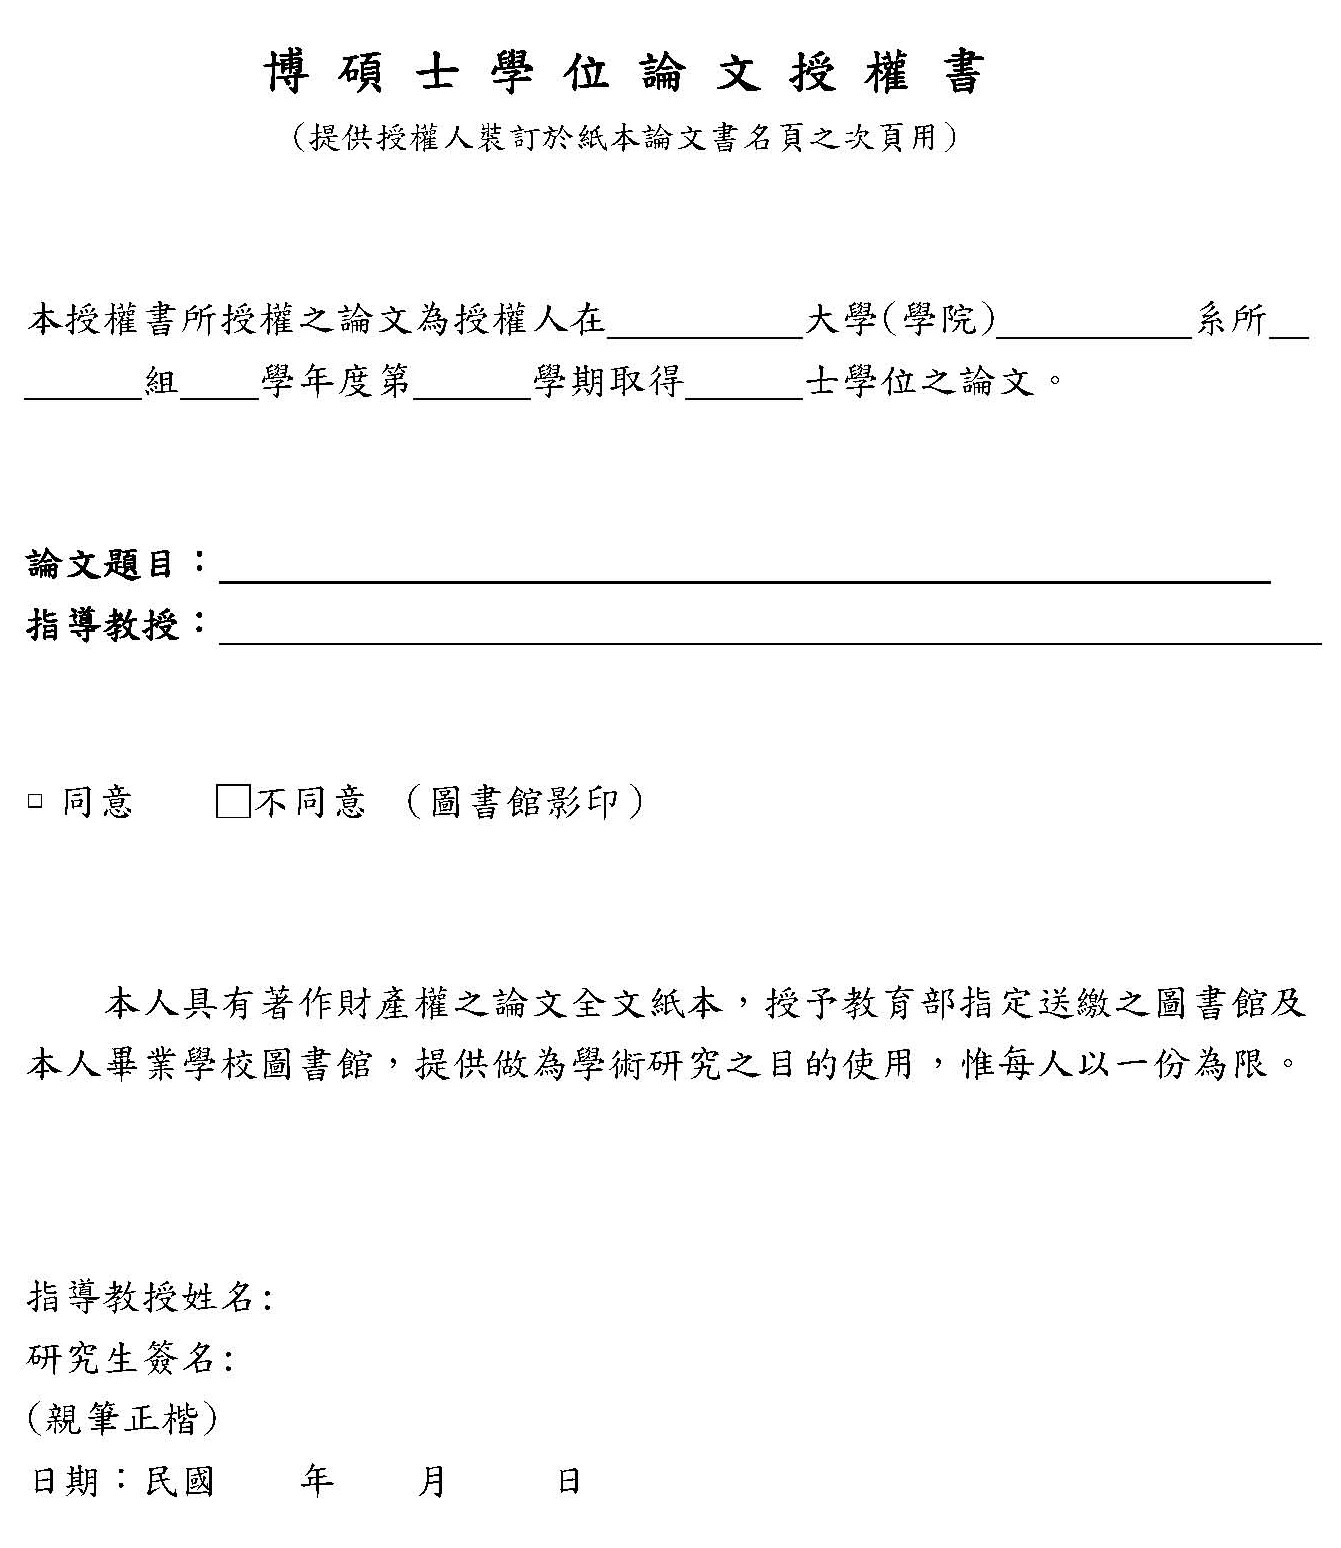
\includegraphics[bb=0 0 1341 1548,width=\textwidth]{authority.jpg}
\end{center}


% 誌謝辭
% \newpage

\begin{center}
    {\LARGE{誌謝辭}}
\end{center}
% 這裡寫上你的誌謝辭內容


% 中文摘要
\newpage
\frontmatter
\begin{center}
    {\LARGE{中文摘要}}
\end{center}
% 中文摘要的內容


% 英文摘要

\newpage
\begin{center}
    {\LARGE SUMMARY}
\end{center}
% 英文摘要的內容


% 目次
\newpage

\tableofcontents

% 表目次
\newpage

\listoftables
% 圖目次
\newpage

\listoffigures

\mainmatter
\setcounter{page}{1} 
\pagenumbering{arabic}  

% 章節
\chapter{一、第一章標題}
% 這裡是第一章的內容
 
\chapter{二、第二章標題}

\chapter{三、第三章標題}
% 這裡是第一章的內容

% 繼續添加其他章節...

\backmatter

% 參考文獻
\backmatter
\chapter{參考文獻}
\renewcommand{\labelenumi}{[\arabic{enumi}]}
\begin{enumerate}
    \item 吳聰敏.吳聰慧(2005), 《cwTEX排版系統》,台北。
    % \item Bringhurst, Robert (1996), {\it The Elements of Typographic Style}, Vancouver: Hartley \& Marks, 2nd edition.
\end{enumerate}


% 附錄
\appendix
\chapter{附錄一 : 封面樣式(一)}
    \begin{center}
        % 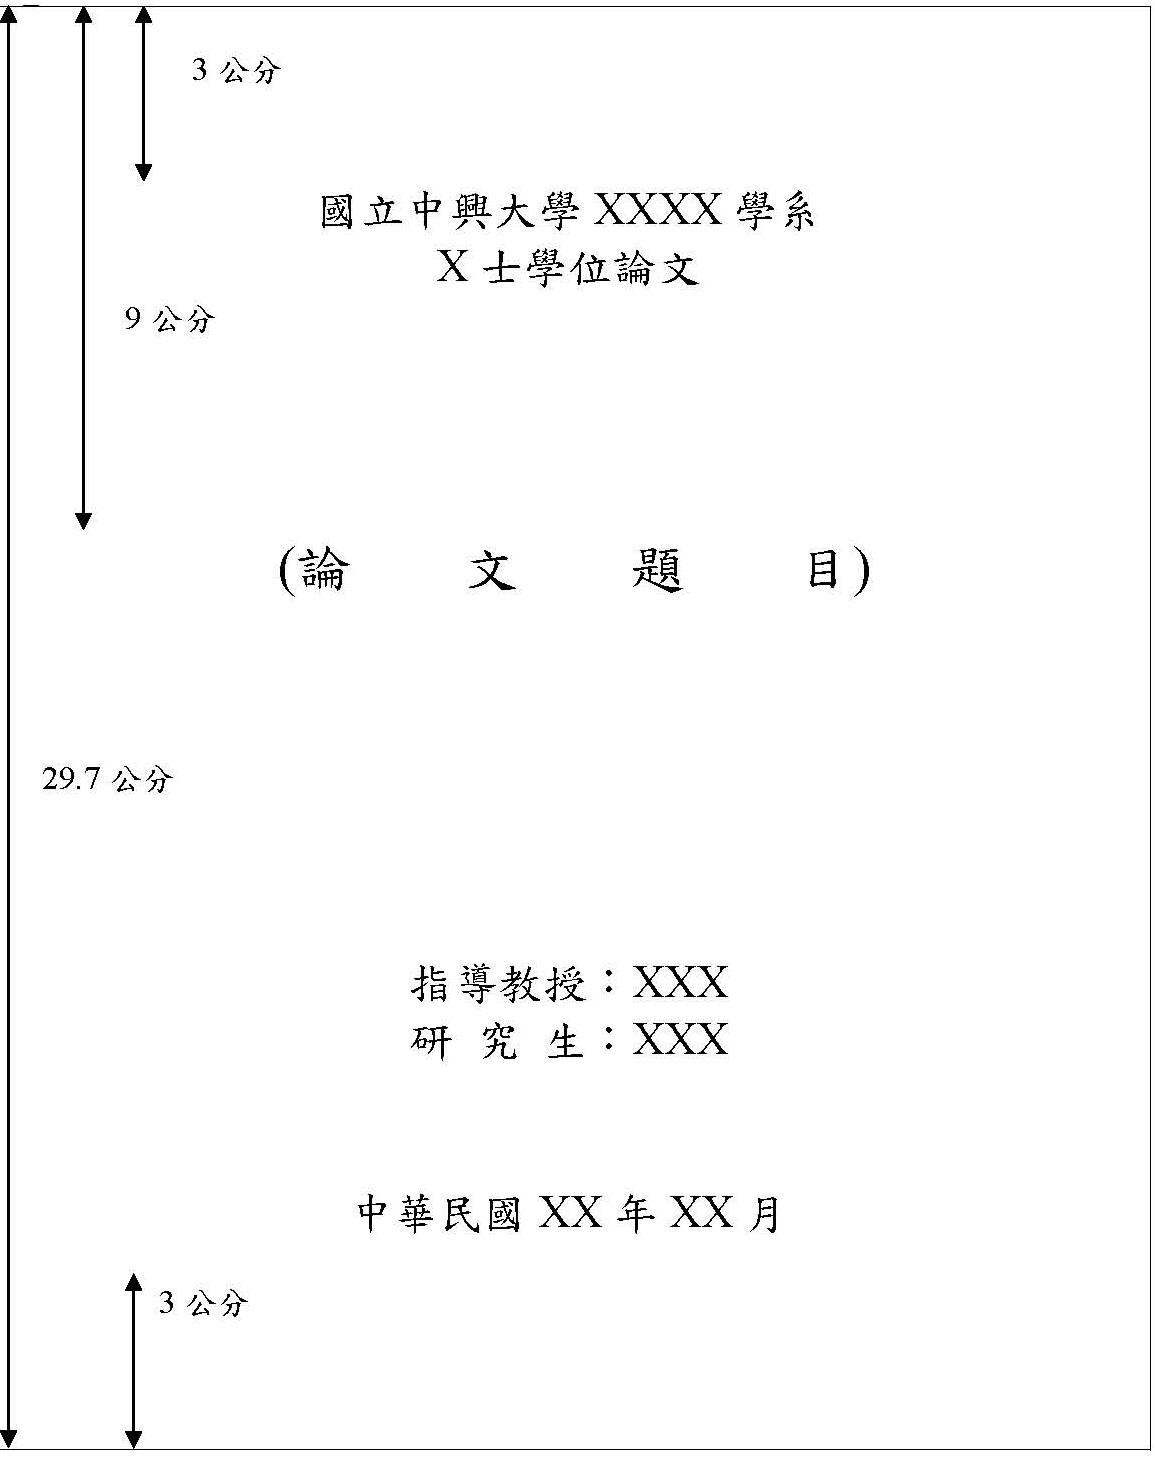
\includegraphics[bb=0 0 1155 1460,width=\textwidth]{TitlePage1.jpg}
    \end{center}

% \include{AppendixB}

\end{document}
